\documentclass[tikz, border=10pt]{standalone}
\usetikzlibrary{patterns}
\usepackage[outline]{contour}
\contourlength{0.09em}

\tikzset{
  nodeAll/.style={draw, rounded corners=3pt, text width=1.5em, align=center, thick},
  nodeA/.style={fill=black, text=white},
  nodeB/.style={fill=white, text=black, pattern=north east lines}
}

\begin{document}

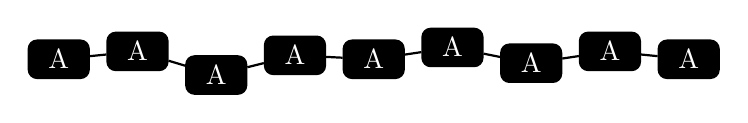
\begin{tikzpicture}
  \node[nodeAll, nodeA] (HP-5) at (-5,0) {A};
  \node[nodeAll, nodeA] (HP-4) at (-4,0.1) {A};
  \node[nodeAll, nodeA] (HP-3) at (-3,-0.2) {A};
  \node[nodeAll, nodeA] (HP-2) at (-2,0.05) {A};
  \node[nodeAll, nodeA] (HP-1) at (-1,0) {A};
  \node[nodeAll, nodeA] (HP0) at (0,0.15) {A};
  \node[nodeAll, nodeA] (HP1) at (1,-0.05) {A};
  \node[nodeAll, nodeA] (HP2) at (2,0.1) {A};
  \node[nodeAll, nodeA] (HP3) at (3,0) {A};

  \path[thick]
    (HP-5) edge (HP-4)
    (HP-4) edge (HP-3)
    (HP-3) edge (HP-2)
    (HP-2) edge (HP-1)
    (HP-1) edge (HP0)
    (HP0) edge (HP1)
    (HP1) edge (HP2)
    (HP2) edge (HP3);
\end{tikzpicture}

\end{document}
